In this section we describe briefly the database creation and the graph query search processes of  \textit{Network Method}. We detail our main contributions: A set of new subgraph query search processing algorithms that implement a fast subgraph search algorithm and on a modified $DAG$ data structure. The improved $DAG$ data structure is able to process both subgraph and induced subgraph queries.

\subsection{The \textit{Network Method}}
 
%\begin{figure}
%\centering
%\epsfig{file=dynamic_acyclic_graph.eps, height=2in, width=3.5in}
%\caption{Messmer et al.'s method}
%\label{fig:fig100}
%\end{figure}

\begin{figure}
\centering
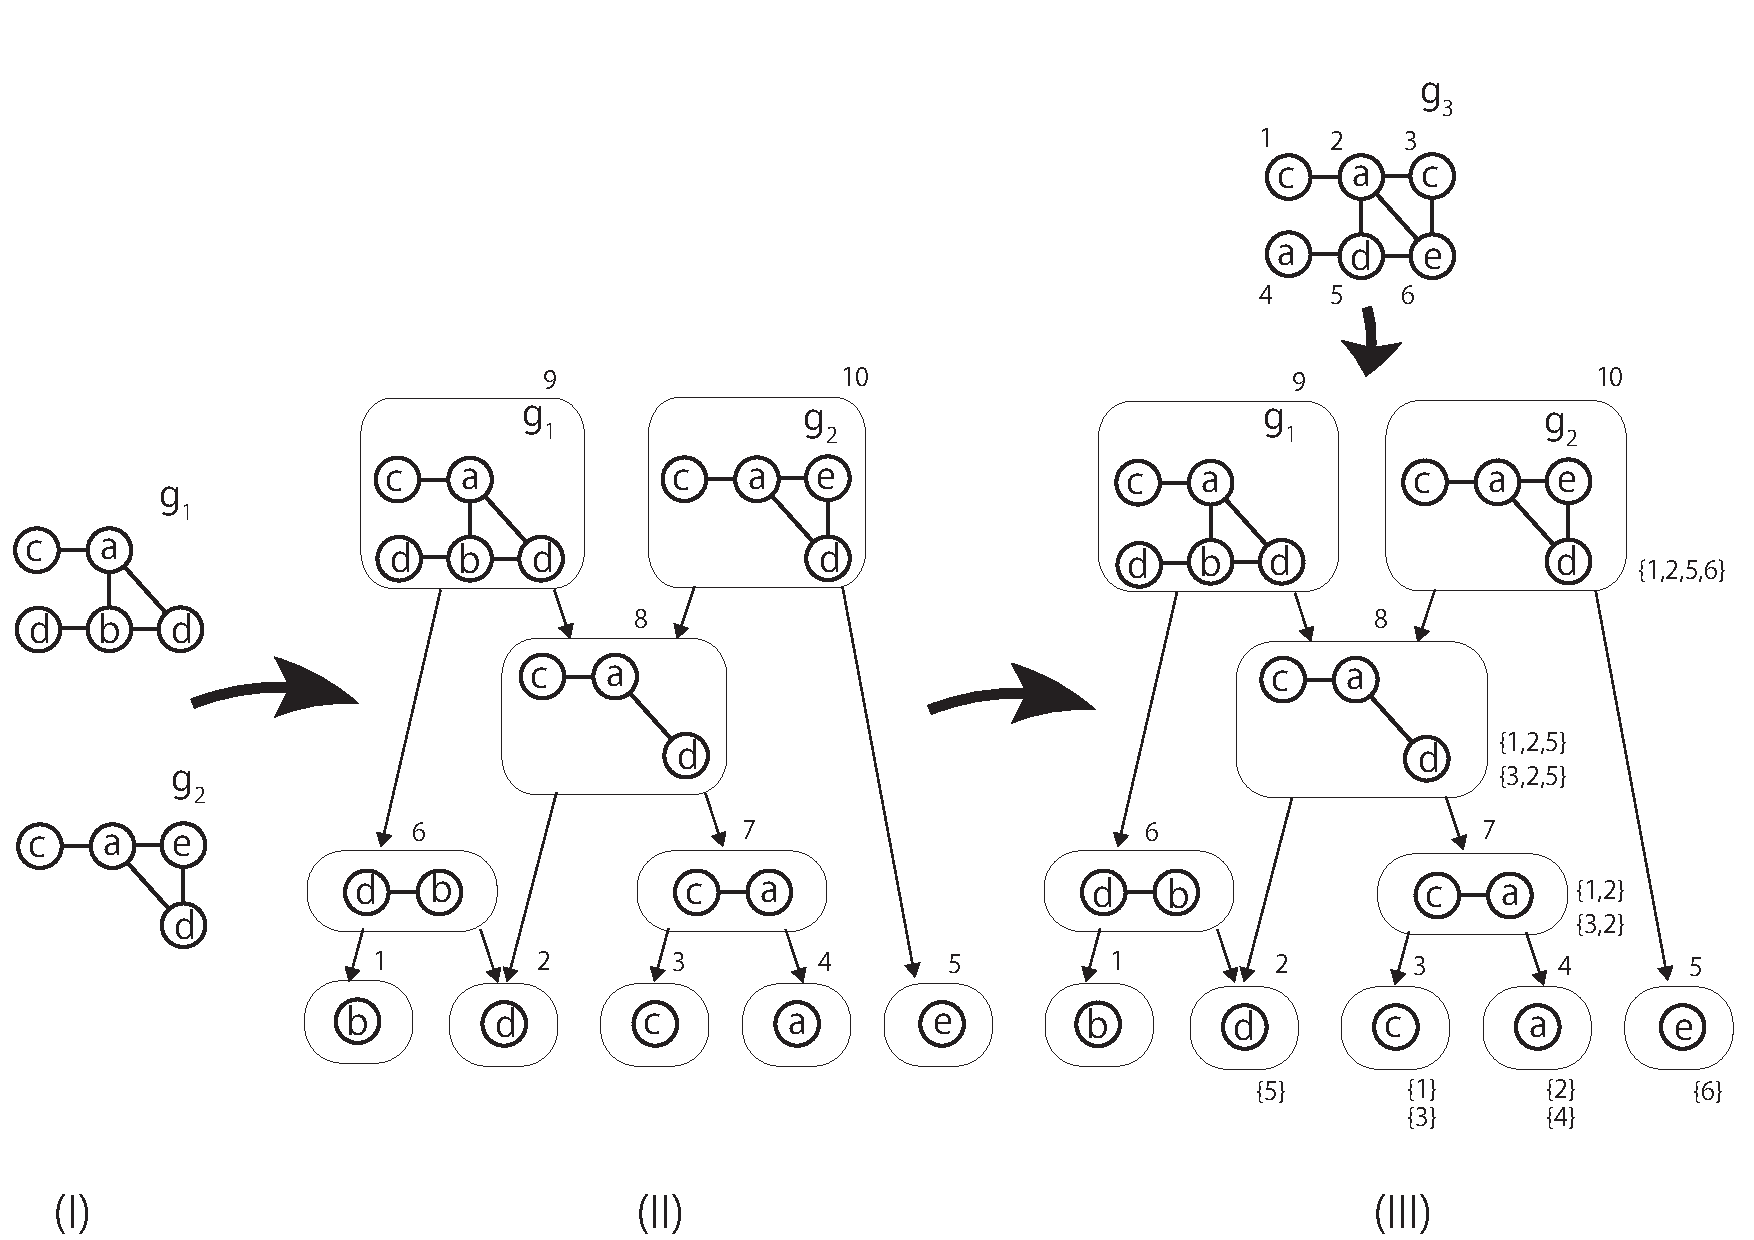
\includegraphics[width=1.0\textwidth]{dag_construction_query_processing6.pdf}
\caption{Schematic of the \textit{Network Method}: (I) Model Graphs $g_1$ and $g_2$, (II) The Graph Database:A DAG is Constructed using  the model graphs $g_1$ and $g_2$ and their decomposed subgraphs. $DAG$ $node$ $8$ contains a subgraph common to model graphs $g_1$ and $g_2$  (III) Query Processing: Query Graph $g_3$ processed on the Graph Database and the matching query graph node IDs shown in braces}
\label{fig:fig2}
\end{figure}


Messmer et al.\cite{messmer_bunke2000} proposed a method to search graphs that are induced subgraphs of a query graph from a graph database. 
Central to the method is a $DAG$ data structure that is used to store decomposed subgraphs of a graph database in a compact form. 
Messmer called this data structure a network so here we will refer to their method as the \textit{Network Method}. 
A simplified schematic of the Network Method is shown in fig.\ref{fig:fig2}. 
This method finds all induced subgraph isomorphisms from graphs in the graph database to a query graph.
We divide the \textit{Network Method} into two parts.

In the first part a directed acyclic graph $DAG$ is constructed by recursively decomposing model graphs and storing the decomposed graphs at the nodes of the $DAG$.
In the $DAG$, the creation of the decomposed graph is directed by the original graph and on decomposition the directed graph is a \textit{child} graph and the directing graph is the \text{parent} graph. 
Fig.\ref{fig:fig2} (II) shows an example of two model graphs that are decomposed and stored in the nodes of a $DAG$ to form a database in (II). A query is processed on this database in (III).
In the process of decomposition, Model graphs $g_1$ and $g_2$ are decomposed into two graphs each, in such a way that each pair of decomposed graphs have as close to equal number of vertices  as possible.
Each of the decomposed pair of graphs is further decomposed into two graphs.
This process continues until the decomposition results in singleton graphs.
Before any graph is decomposed, it is checked for containment of an induced subgraph previously created by the decomposition process so far. If one is found, the graph is decomposed into the induced subgraph and a rest subgraph. In this way, an induced subgraph can be shared by multiple parents as shown in Fig.\ref{fig:fig2} where $g_1$ is decomposed randomly into subgraph $6$ and subgraph $8$ by partitioning approximately an equal number of vertices.
If $g_2$ contains an induced subgraph $8$, $g_2$ is decomposed into graph $8$ and graph $5$ after the all decomposition of $g_1$ has finished.

In the second part an induced subgraph isomorphism query is processed using the $DAG$ constructed in first part.
First, all induced subgraph isomorphisms from all singleton graphs in the $DAG$ to query graph are detected.
Based on the induced subgraph isomorphisms, induced subgraph isomorphisms of the respective parent graphs are calculated by combining the induced subgraph isomorphisms of its child graphs. This process repeats until finally, all induced subgraph isomorphisms of model graphs to the query are detected.
The \textit{Network Methood} makes use of the fact that if a graph in $DAG$ is not an induced subgraph of query graph, its ancestors are also not induced subgraphs.
In Fig.\ref{fig:fig2} part(III), if \textit{node 8} is not an induced subgraph of $g_3$, we know each of $g_1$ and $g_2$ are also not induced subgraph of $g_3$without performing any additional computation. Using this knowledge the time required to process the induced subgraph query is reduced by avoiding this unnecessary computation. The main advantages of the \textit{Network Algorithm}  are:  

\begin{enumerate}
\item The $DAG$ is constructed by decomposing graphs recursively which allows efficient solution of queries by divide and conquer.
\item The induced subgraph isomorphisms of induced subgraphs discovered in the $DAG$ that are common to multiple model graphs are computed only once and the result is shared.
\end{enumerate}

\subsection{Our Contributions}
We have two main contributions. 
First, we propose a new search strategy for the graph database that can be used for both induced and non-induced subgraphs. 
We use this new algorithm to implement a framework for fast and scalable graph database creation and subgraph query processing. 
Secondly, we propose modifications to the $DAG$ data structure to enable processing both subgraph query search and induced subgraph query search on the modified $DAG$ data structure. 


We implement these proposals in a framework where we create a graph database and evaluate the performance of subgraph isomorphism query search on the database. This is different from \textit{Network Method} which can only processes induced subgraph isomorphism queries. 


We observe an order of magnitude improvement in processing time over the state-of-the-art isomorphism test algorithm VF2.  
We also evaluate the performance of induced subgraph query search. Here we observe several orders of magnitude improvement in processing time over the \textit{Network Method} and an order of magnitude improvement over VF2 for random graphs. 
We call the new framework for database creation and subgraph search \textit{Fast Network Method}. 
The details of the proposed \textit{Fast Network Method} are described below where we contrast it with the \textit{Network Method}.


%\begin{figure}[t]
%\centering
%\epsfig{file=partition.eps, height=2.3in, width=3in}
%\caption{Two ways to decompose a graph into two subgraphs}
%\label{fig:fig2}
%\end{figure}



\begin{figure}
\centering
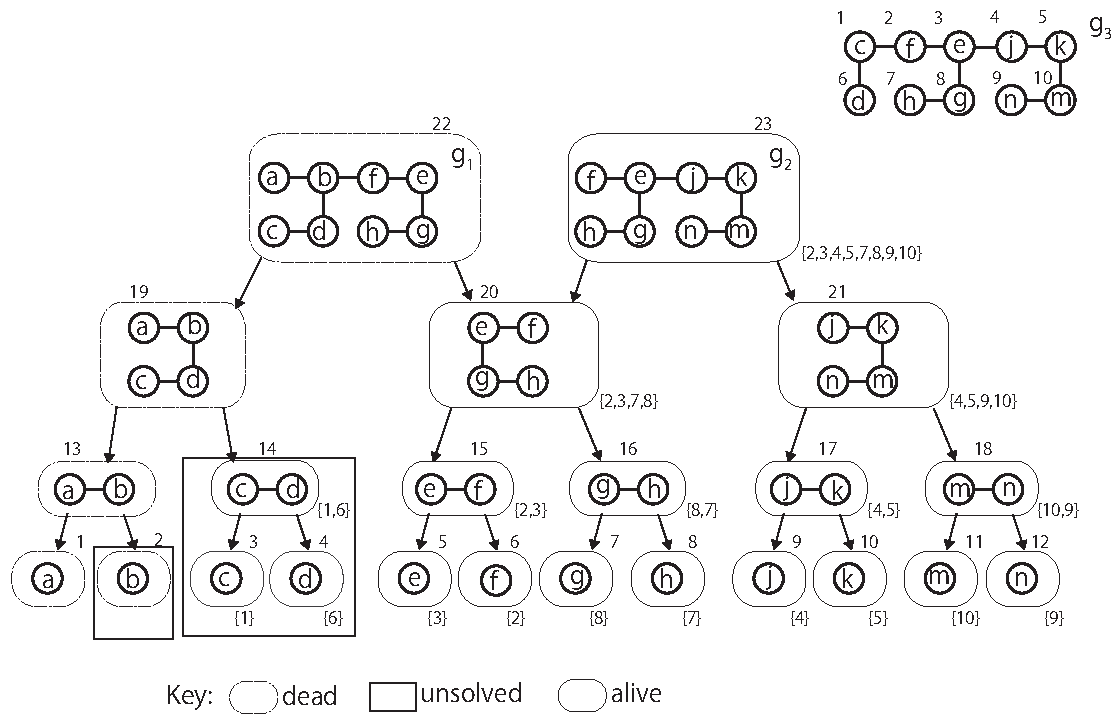
\includegraphics[width=1.0\textwidth]{dag_search_optimize.pdf}
\caption{The search strategy for the \textit{New Network Algorithm}: For a simplified database composed of model graphs $g_1$ and $g_2$, given a query graph $g_3$ each model graph is processed locally by starting at the top of the $DAG$ in a depth first search (DFS) fashion. 
The search concludes when the first \textit{dead} state is encountered. 
Specifically, we conclude that nodes 1,13,19, 22 (hence model graph $g_1$) are in \textit{dead} state as soon as node 1 is processed. 
After processing $g_1$ and $g_2$ we have the result in spite of nodes 2,3,4, and 14 remaining in \textit{unsolved} state. 
In contrast, the \textit{Network Algorithm} processes \textit{all} the nodes in the $DAG$ in the order of the numbers on the top right of the nodes before any output is delivered.}
\label{fig:fig3}
\end{figure}

\begin{figure}
        \centering
        %& -shell-escape -enable-write18
\documentclass{standalone}
\usepackage{tikz}
\usetikzlibrary{matrix}
\usetikzlibrary{shapes,arrows}
\usepackage{caption}

%\newcommand{mynodename}[#1]{\mathrm{#1}}
%\newcommand{mylabelleft}[#2]{label={[font=\fontsize{#1}{#1}\selectfont]above left:mynodename{#2}}}
\begin{document}

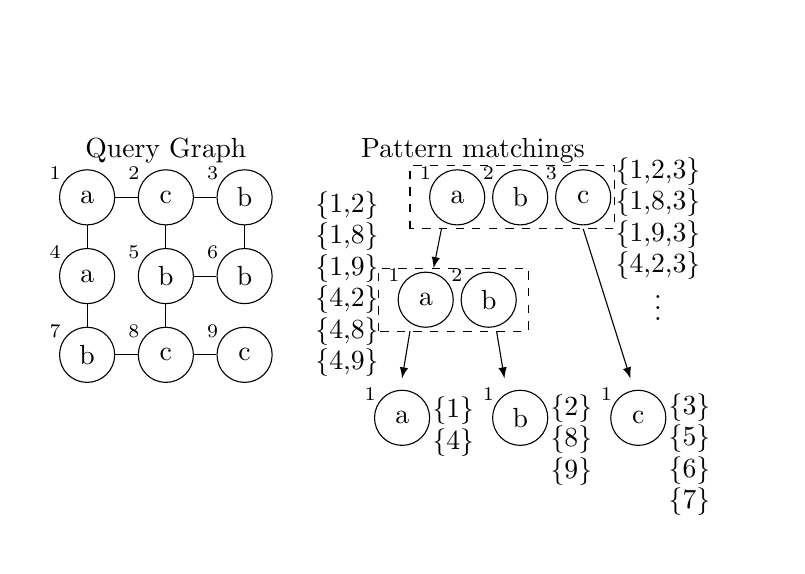
\begin{tikzpicture}[scale=1.0]
%[every node/.style={draw,circle}]
\tikzstyle{every node}=[draw,shape=circle,minimum size=0.7cm];
\tikzstyle{mylabels}=[font=\fontsize{7}{7}\selectfont,yshift=-.2cm];
\tikzstyle{line} = [draw,-latex];
\tikzstyle{dashedline} = [draw,dashed];
\colorlet{invisible}{white}
\colorlet{visible}{black}

\begin{scope}[shift={(.3,.3)}]
%\draw[help lines,step=.2cm] (-1,-6) grid (10,6);;
  \node (n1) at (0,2) [label={[font=\fontsize{7}{7}\selectfont,xshift=.1cm,yshift=-.2cm]above left:$1$}] {a};
  \node (n2) at (1,2) [label={[font=\fontsize{7}{7}\selectfont,xshift=.1cm,yshift=-.2cm]above left:$2$}] {c};
  \node (n3) at (2,2) [label={[font=\fontsize{7}{7}\selectfont,xshift=.1cm,yshift=-.2cm]above left:$3$}] {b};
  \node (n4) at (0,1) [label={[font=\fontsize{7}{7}\selectfont,xshift=.1cm,yshift=-.2cm]above left:$4$}] {a};
  \node (n5) at (1,1) [label={[font=\fontsize{7}{7}\selectfont,xshift=.1cm,yshift=-.2cm]above left:$5$}] {b};
  \node (n6) at (2,1) [label={[font=\fontsize{7}{7}\selectfont,xshift=.1cm,yshift=-.2cm]above left:$6$}] {b};
  \node (n7) at (0,0) [label={[font=\fontsize{7}{7}\selectfont,xshift=.1cm,yshift=-.2cm]above left:$7$}] {b};
  \node (n8) at (1,0) [label={[font=\fontsize{7}{7}\selectfont,xshift=.1cm,yshift=-.2cm]above left:$8$}] {c};
  \node (n9) at (2,0) [label={[font=\fontsize{7}{7}\selectfont,xshift=.1cm,yshift=-.2cm]above left:$9$}] {c};
  
  \node [draw=none] (query_label) at (1,2.6) {Query Graph};% query graph label

  \foreach \from/\to in {n1/n2,n2/n3,n1/n4,n5/n6,n2/n5,n3/n6,n4/n7,n7/n8,n5/n8,n8/n9}
    \draw (\from) -- (\to);
\end{scope}

\begin{scope}[shift={(5,0)}]
	\begin{scope}[shift={(0,0.3)}]%top  row
		\node (n10) at (0,2) [label={[font=\fontsize{7}{7}\selectfont,xshift=.1cm,yshift=-.2cm]above left:$1$}] {a};
		\node (n11) at (.8,2) [label={[font=\fontsize{7}{7}\selectfont,xshift=.1cm,yshift=-.2cm]above left:$2$}] {b};
		\node (n12) at (1.6,2) [label={[font=\fontsize{7}{7}\selectfont,xshift=.1cm,yshift=-.2cm]above left:$3$}] {c};
		\draw[dashedline] (-.6,1.6) rectangle (2,2.4);
		
		\path[line] (-.2,1.6) -- (-.3,1.1);%left side
		\path[line] (1.6,1.6) -- (2.2,-.3);%long arrow on right side

		\node [draw=none] (patternmatching_label) at (.2,2.6) {Pattern matchings};% query graph label
	\end{scope}
	\begin{scope}[shift={(-.4,0)}] %middle row
		\node (n13) at (0,1)  [label={[font=\fontsize{7}{7}\selectfont,xshift=.1cm,yshift=-.2cm]above left:$1$}] {a};
		\node (n14) at (.8,1) [label={[font=\fontsize{7}{7}\selectfont,xshift=.1cm,yshift=-.2cm]above left:$2$}] {b};
		\draw[dashedline] (-.6,.6) rectangle (1.3,1.4);
		\path[line] (-.2,0.6) -- (-.3,0);
		\path[line] (.9,0.6) -- (1,0);
	\end{scope}
	\begin{scope}[shift={(-.7,-.5)}] %bottom row
		\node (n15) at (0,0) [label={[font=\fontsize{7}{7}\selectfont,xshift=.1cm,yshift=-.2cm]above left:$1$}] {a};
		\node (n16) at (1.5,0) [label={[font=\fontsize{7}{7}\selectfont,xshift=.1cm,yshift=-.2cm]above left:$1$}] {b};
		\node (n17) at (3,0) [label={[font=\fontsize{7}{7}\selectfont,xshift=.1cm,yshift=-.2cm]above left:$1$}] {c};
		
	\end{scope}

  \foreach \from/\to in {n1/n2,n2/n3,n1/n4,n5/n6,n2/n5,n3/n6,n4/n7,n7/n8,n5/n8,n8/n9}
    \draw (\from) -- (\to);
\end{scope}
\begin{scope}[shift={(7.5,1.8)}]
			\matrix (m)[matrix of nodes, column  sep=-1mm,color=visible,row  sep=-3mm, anchor=center,draw=none,nodes={rectangle,color=invisible,draw=none}]{ %,text width = 2cm
\node [color=visible] {\{1,2,3\}};&\\
\node[color=visible] {\{1,8,3\}};& \\
\node[color=visible] {\{1,9,3\}};& \\
\node[color=visible] {\{4,2,3\}};& \\
\node[color=visible] {\vdots};& \\
	};
\end{scope}
\begin{scope}[shift={(3.55,1.2)}]
			\matrix (m)[matrix of nodes, column  sep=-1mm,color=visible,row  sep=-3mm, anchor=center,draw=none,nodes={rectangle,color=invisible,draw=none}]{ %,text width = 2cm
\node [color=visible] {\{1,2\}};&\\
\node[color=visible] {\{1,8\}};& \\
\node[color=visible] {\{1,9\}};& \\
\node[color=visible] {\{4,2\}};& \\
\node[color=visible] {\{4,8\}};& \\
\node[color=visible] {\{4,9\}};& \\
	};
\end{scope}
\begin{scope}[shift={(4.9,.2)}]
			\matrix (m)[matrix of nodes, column  sep=-1mm,color=visible,row  sep=-3mm, anchor=north,draw=none,nodes={rectangle,color=invisible,draw=none}]{ %,text width = 2cm
\node [color=visible] {\{1\}};&\\
\node[color=visible] {\{4\}};& \\
	};
\end{scope}
\begin{scope}[shift={(6.4,.2)}]
			\matrix (m)[matrix of nodes, column  sep=-1mm,color=visible,row  sep=-3mm, anchor=north,draw=none,nodes={rectangle,color=invisible,draw=none}]{ %,text width = 2cm
\node [color=visible] {\{2\}};&\\
\node[color=visible] {\{8\}};& \\
\node[color=visible] {\{9\}};& \\
	};
\end{scope}
\begin{scope}[shift={(7.9,.2)}]
			\matrix (m)[matrix of nodes, column  sep=-1mm,color=visible,row  sep=-3mm, anchor=north,draw=none,nodes={rectangle,color=invisible,draw=none}]{ %,text width = 2cm
\node [color=visible] {\{3\}};&\\
\node[color=visible] {\{5\}};& \\
\node[color=visible] {\{6\}};& \\
\node[color=visible] {\{7\}};& \\
	};
\end{scope}
\end{tikzpicture}

\end{document}
        \caption{An example of the explosion of number of matchings \label{fig:fig4} }
\end{figure}

\begin{table}
\begin{center}\begin{tabular}{|c|c|c|}
\hline
  & Vertex partition  & Edge partition  \\ \hline
Subgraph & sometimes infeasible  & feasible \\ \hline
Induced subgraph & feasible & sometimes  infeasible \\ \hline
\end{tabular}
\caption{Appropriate method for decompositions \label{tab:table1} }
\end{center}
\end{table}

\begin{figure}
\centering
%& -shell-escape -enable-write18
\documentclass{standalone}
\usepackage{tikz}
%\usepackage{caption}
\usetikzlibrary{external}
\usetikzlibrary{shapes,arrows}
%\newcommand{mynodename}[#1]{\mathrm{#1}}
%\newcommand{mylabelleft}[#2]{label={[font=\fontsize{#1}{#1}\selectfont]above left:mynodename{#2}}}
\begin{document}
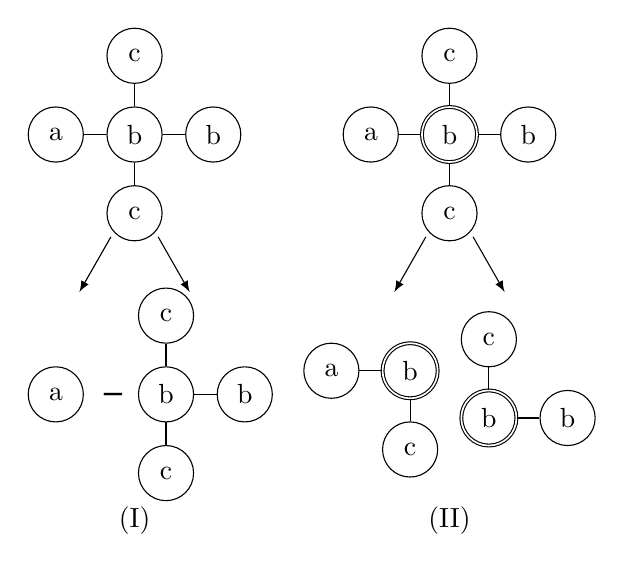
\begin{tikzpicture}[scale=1.0]
%[every node/.style={draw,circle}]
\tikzstyle{every node}=[draw,shape=circle,minimum size=0.7cm];
\tikzstyle{mylabels}=[font=\fontsize{7}{7}\selectfont];
\tikzstyle{line} = [draw,-latex]


%\draw[help lines] (-1.0,-6.0) grid (12.0,6.0);
\begin{scope}[shift={(0,0)}]%upper row set
	\begin{scope}[shift={(1,4.0)}]%upper row left
  		\node (a1) at (0,0) {a};
 		\node (b1) at (1,0) {b};
  		\node (b2) at (2,0) {b};
  		\node (c1) at (1,1) {c};
  		\node (c2) at (1,-1) {c};
  
		\foreach \from/\to in {a1/b1,b1/b2,b1/c1, b1/c2}
   		 \draw (\from) -- (\to);
	\end{scope}
	\begin{scope}[shift={(5.0,4)}]%upper row right
 		 \node (a2) at (0,0) {a};
 		 \node[draw,double,shape=circle,minimum size=0.7cm] (b3) at (1,0) {b};
 		 \node (b4) at (2,0) {b};
		 \node (c3) at (1,1) {c};
 		 \node (c4) at (1,-1) {c};
  
	  	\foreach \from/\to in {a2/b3,b3/b4,b3/c3, b3/c4}
   		 \draw (\from) -- (\to);
	\end{scope}
\end{scope}%upper row set
\begin{scope}[shift={(0,0.7)}]% lower row set
	\begin{scope}[shift={(0,0)}] % lower row extreme left
		\node (a3) at (1,0) {a};
		\node [draw=none] (minus)      at   (1.6,0){\scalebox{2.5}[1.5]{ -} };%horizontal scaling with no vertical scaling
		\node [draw=none] (EdgeCutting) at (2.0,-1.6) { (I) };% edge cutting label
		\node [draw=none] (EdgeCutting) at (6.0,-1.6) { (II) };% edge cutting label
	\end{scope}
	\begin{scope}[shift={(2.4,0)}]%lower row second from left
  		\node (b5) at (0,0) {b};
 		\node (b6) at (1,0) {b};
		\node (c5) at (0,1) {c};
		\node (c6) at (0,-1) {c};
		
		
		\foreach \from/\to in {b5/b6,b5/c5, b5/c6}
			\draw (\from) -- (\to);
	\end{scope}
	\begin{scope}[shift={(4.5,.3)}]% lower row middle right
  		\node (a4) at (0,0) {a};
  		\node[draw,double,shape=circle,minimum size=0.7cm] (b7) at (1,0) {b};
  		\node (c7) at (1,-1) {c};
  
 		 \foreach \from/\to in {a4/b7,b7/c7}
   		 \draw (\from) -- (\to);
	\end{scope}% lower row middle right
	\begin{scope}[shift={(5.5,-.3)}]% lower row extreme right
		\node[draw,double,shape=circle,minimum size=0.7cm] (b8) at (1,0) {b};
		\node (b9) at (2,0) {b};
 		\node (c8) at (1,1) {c};
 	 		\foreach \from/\to in {b8/b9,b8/c8}
	    		\draw (\from) -- (\to);
	\end{scope}% lower row extreme right
\end{scope}%lower row set
\begin{scope}[shift={(0,0)}]% the arrows set
	\begin{scope}[shift={(1.8,2.7)}]%the left arrows
		\path[line] (-0.1,0) -- (-0.5,-0.7);
		\path[line] (0.5,0) -- (0.9,-0.7);
	\end{scope}
	\begin{scope}[shift={(5.8,2.7)}]%the right arrows
		\path[line] (-0.1,0) -- (-0.5,-0.7);
		\path[line] (0.5,0) -- (0.9,-0.7);
	\end{scope}
\end{scope}
\end{tikzpicture}
\end{document}

\caption{Two ways to decompose a graph, (I) \textit{Decomposition to induced subgraph} by partitioning the set vertices (interconnecting edge cutting). (II) \textit{Decomposition to subgraph} by partitioning the set of edges (common vertex sharing).}
\label{fig:fig55}
\end{figure}

\begin{enumerate}

\item A Fast Search Strategy for graph database Search

The search strategy works by minimizing the search space as follows.
\begin{enumerate}
\item{Localized subgraph Search}

As shown in Fig.\ref{fig:fig3} for each model graph in the database, the search process begins at the top, say $g_1$ and proceeds recursively in a depth first search(DFS) fashion until the state of the present node is in \textit{unsolved} or \textit{dead} state, or until the subgraph at the node is a singleton. When a node in \textit{dead} state is encountered, the processing terminates and the current model graph assigned \textit{dead} state. This is different from the \textit{network method} where the search proceeds by first processing all leaf nodes in the $DAG$. It then proceeds to the second level in the $DAG$ in the order of the number on top of the nodes till the model graphs at the top of the $DAG$ are reached. Only after processing the nodes in the $DAG$ is the isomorphism of the model graphs determined for those that are in  \textit{alive} state. As a consequence, processing of the whole $DAG$ continues regardless of some of the subgraphs being determined to be in \textit{dead} state.

By localizing subgraph search, the minimum processing required to determine a Model Graph to be in \textit{dead} state is processing of a single singleton mode. This case is illustrated in Fig.\ref{fig:fig3} where node 1 is found to be in \textit{dead} state on processing.


Once the state of a subgraph of the model graph is determined to be \textit{dead}, further subgraph isomorphism processing terminates. This usually results in some subgraphs of the model graph remaining in unprocessed state which is a very desirable situation as a unnecessary computation effort is avoided. In the case of \ref{fig:fig3} node 2,3,4,and 14 remain in \textit{unsolved state} while the model graph $g_1$ is determined to be in \textit{dead} state, hence not subgraph isomorphic to the query graph $g_3$.

\item{Rapid propagation of subgraph search state}

To process a query over a graph database, the query is performed for each model graph stored in the $DAG$. 
The processing subgraph matchings for isomorphism for each model graph terminates as soon a non-isomorphic subgraph that is, a \textit{dead} state, is encountered or the model graph is found to be isomorphic. 


On termination, all the ancestors of the non-isomorphic subgraph are set to \textit{dead} state. In Fig.\ref{fig:fig3} the label for node 1 does not appear in $g_3$ therefore the node is not a match. It is in \textit{dead} state. Since we arrived at node 1 by repeated recursive calls from nodes 13, 19 and 22, we return the \textit{dead} state to each of these nodes as the recursion terminates. This is the process of Rapid Propagation of the subgraph state to the Model graph that enables early discovery of the state of common subgraphs. When t

By processing each model graph to completion, the \textit{Fast Network Algorithm} is potentially more efficient as the state of larger common subgraphs is known with each model subgraph. When the shared larger subgraph is non isomorphic to the query, the potential search space is reduced significantly.



The \textit{Network Algorithm} searches all nodes in $DAG$ from the leaf nodes in a bottom up fashion.
As a result, all the child nodes in the $DAG$ will get processed before the parent nodes. 
The state of the parent nodes is computed after all the child nodes have been computed. 
This results in some unnecessary computation in the case that one or more of the children are found not to be isomorphic to a query because a parent graph state determined as non isomorphic if at least one children is not isomorphic to a query.  
In fact when the isomorphism state is negative, only one test is sufficient to discover the state of all the ancestral graphs. 
We use a simple example in Fig.\ref{fig:fig2} (III) to illustrate this.
Assume that we know that $node$ 6 is not a subgraph of query $g_3$ in advance. 
This implies that $g_1$ is not a subgraph of the query $g_3$.
Hence we need not check $node$ 8 and its descendants to know the status of $g_1$ which we propagate. 
Further, the potential computation savings increase when a non isomorphic subgraph is common to multiple parents. 
We propose a recursive algorithm for subgraph search with state propagation of subgraph status to avoid the needless calculations. 
This results in a \textit{New Network Algorithm} is faster than the \textit{Network Algorithm}.

\end{enumerate}

\item  Subgraph query processing using \textit{Fast Network Method}

\begin{enumerate}

\item Data structure

The data structure used for subgraph storage in both the \textit{Network Method} as well as the \textit{Fast Network Method} consists of a directed acyclic graph($DAG$). 
A simplified schematic of the $DAG$ is show in Fig.\ref{fig:fig2}. 
The nodes in the $DAG$ represent decomposed subgraphs of the model graphs that are stored in a database. 
only implements only processing of induced subgraph queries. 
We implement an extension of the method enable processing of subgraph queries. 
This limitation in the \textit{Network Algorithm} occurs due to the method of decomposition by vertex partition used to facilitate induced subgraph isomorphism query. 
A provision is required for a similar facility suited to subgraph isomorphism query. 
To do so, we use the algorithms intended for processing induced subgraphs, mostly by replacing the term \textit{induced subgraph} with \textit{subgraph} in the next section.
Then, we define a new decomposition method by partitioning edges, that is suited for processing subgraphs.


Table. \ref{tab:table1} summarizes feasible approaches to decomposition. 
In the \textit{Network Algorithm}, graphs are decomposed by partitioning vertices (cutting edges).
In order to extend the \textit{Network Algorithm} to non-induced subgraph query, we implement \textit{decomposition to subgraph} by partitioning edges (shared vertices). 
Fig.\ref{fig:fig55} shows the difference between two methods of decomposition. 
We now describe the rationale for the difference in decomposition described above.

For induced subgraph query, we have to decompose a graph partitioning vertices to form two induced subgraphs and store the information about the interconnecting cut edges. 
Both the resulting children must be induced subgraphs of their parent to enable the processing of induced subgraph queries in a divide and conquer fashion. 
However, Decomposing an arbitrary graph into its induced subgraph and rest graph by shared vertices such that both children are induced subgraphs of the parent cannot be assured.

In Fig.\ref{fig:fig66} we see an example where the decomposition of a graph into two induced subgraphs is infeasible by partitioning edges (sharing vertices).
If we decompose $g$ by partitioning edges, the rest graph is $s_{rest}$. But $s_{rest}$ must be an induced subgraph of $g$, so the edge is complemented as $s_{rest}'$ and $s_{rest}'$ is equal to $g$. 
This indicates that we cannot decompose a graph $g$ any further as $g$ is a complete graph.
The subtraction of induced subgraph by partitioning vertices (vertex subtraction)  is defined in \textit{Definition \ref{def:def37}}.

For subgraph query, we need to decompose graphs by partitioning edges. 
This is due to the requirement that both children must be subgraphs of their parent graphs
and the limitation that we are unable to decompose a graph into an arbitrary subgraph and the rest graph by partitioning vertices so that rest graph becomes subgraph of its parent.
Fig.\ref{fig:fig7} shows an example where a decomposition of a graph into two subgraphs is not feasible by partitioning vertices.
If we subtract $s$ from $g$ by partitioning vertices, $s_{rest}$ cannot be represented as a graph as only an edge remains. 
We need to subtract the subgraphs by partitioning edges and then including the vertices on the edges as $s_{rest}'$ shows. 
Hence subgraph query processing we decompose the graphs by partitioning edges and including the corresponding vertices.
The subtraction of subgraphs by partitioning edges (edge subtraction)is defined in \textit{Definition \ref{def:def310}}.

We use the appropriate decomposition for both decompositions and also reform corresponding algorithms.

\item Subgraph processing algorithms

In addition to the specialized routines for subgraph decomposition mentioned in the previous section,  we have also developed a parallel set of routines for both the construction of the $DAG$ and query processing. 

%% Non induced subgraphs can only be decomposed by shared vertices  
\end{enumerate}


\item Induced subgraph query processing

\begin{enumerate}
\item Decomposing a graph into two connected subgraphs.

The \textit{Network Algorithm} decomposes a graph at random and without any restriction on the resulting subgraphs other than that they be connected graphs.
Therefore the decomposition result possibly creates multiple connected graph composed of many small graph fragments.
However the number of matchings from number of smaller graphs to a query graph can easily become intractable.
Fig.\ref{fig:fig4} shows an extreme example of the rapid increase of the matchings that results when a graph is decomposed to singletons.
The number of matchings correlate with processing time as well as memory requirements, hence the need to restrict them. We reformulate the decomposition algorithm with the restriction that a connected graph must be decomposed to strictly result in only two connected subgraphs. When decomposition results in one or both graph disconnected, we post-process the resulting subgraphs by redistributing one or both components between the children  at random until two connected graphs result.

%\begin{figure}
%\centering
%\epsfig{file=images/explosion.eps, height=2.2in, width=3.5in}
%\caption{An example of the explosion of number of matching}
%\label{fig:fig102}
%\end{figure}

\item Early propagation of subgraph search state.

The \textit{Network Algorithm} searches all nodes in $DAG$ from the leaf nodes in a bottom up fashion.
As a result, all the child nodes in the $DAG$ will get processed before the parent nodes. 
The state of the parent nodes is computed after all the child nodes have been computed. 
This results in some unnecessary computation in the case that one or more of the children are found not to be isomorphic to a query because a parent graph state determined as non isomorphic if at least one children is not isomorphic to a query.  
In fact when the isomorphism state is negative, only one test is sufficient to discover the state of all the ancestral graphs. 
We use a simple example in Fig.\ref{fig:fig2} (III) to illustrate this.
Assume that we know that $node$ 6 is not a subgraph of query $g_3$ in advance. 
This implies that $g_1$ is not a subgraph of the query $g_3$.
Hence we need not check $node$ 8 and its descendants to know the status of $g_1$ which we propagate. 
Further, the potential computation savings increase when a non isomorphic subgraph is common to multiple parents. 
We propose a recursive algorithm for subgraph search with state propagation of subgraph status to avoid the needless calculations. 
This results in a \textit{New Network Algorithm} is faster than the \textit{Network Algorithm}.
\end{enumerate}

%\begin{figure}[t]
%\centering
%\epsfig{file=ex_induced_decomposition.eps, height=0.8in, width=3in}
%\caption{An example that a decomposition of a graph into two induced subgraphs is unable by sharing vertices}
%\label{fig:fig11}
%\end{figure}


\begin{figure}
\centering
git%& -shell-escape -enable-write18
\documentclass{standalone}
\usepackage{tikz}
\usetikzlibrary{external}
%\usepackage{caption}
\usetikzlibrary{shapes,arrows}
\newcommand{\mynodelabelfont}[1]{\fontsize{#1pt}{#1pt}\selectfont,yshift=-.2cm}
%\newcommand{mynodename}[#1]{\mathrm{#1}}

\begin{document}
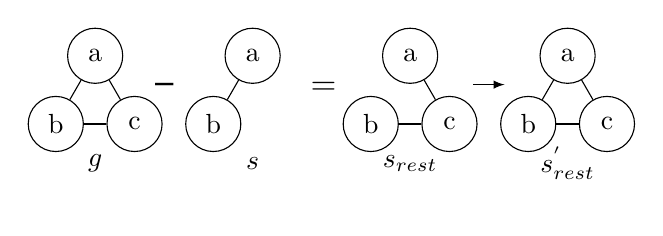
\begin{tikzpicture}[scale=1.0]
%[every node/.style={draw,circle}]
\tikzstyle{myline} = [draw,-latex]
\tikzstyle{every node}=[draw,shape=circle,minimum size=0.7cm];
%\tikzstyle{mylabelsfont=[font=\fontsize{7}{7}\selectfont,yshift=-.2cm];
%\tikzstyle{every label}=[text height=10pt];
\begin{scope}[xshift=0cm]
  \node (a) at (60:1cm) {a};
  \node (b) at (0:0cm)  {b};
  \node (c) at (0:1cm)  {c};
  \node [draw=none] (minus)  at   (1.4,.5){\scalebox{2.5}[1.5]{-} };
  \node [draw=none] (SharedVertices) at (.5,-.5) {$g$};% sharedvertices label


  \foreach \from/\to in {a/b,b/c,c/a}
    \draw (\from) -- (\to);
\end{scope}
\begin{scope}[xshift=2cm]
  \node (a) at (60:1cm) {a};
  \node (b) at (0:0cm)  {b};
  \node [draw=none] (minus)  at   (1.4,.45){\scalebox{1.2}[1.2]{=} };
  \node [draw=none] (SharedVertices) at (.5,-.5) {$s$};%sharedvertices label

  \foreach \from/\to in {a/b}
    \draw (\from) -- (\to);
\end{scope}
\begin{scope}[xshift=4cm]
  \node (a) at (60:1cm) {a};
  \node (b) at (0:0cm)  {b};
  \node (c) at (0:1cm)  {c};
  \node [draw=none] (SharedVertices) at (.5,-.5) {$s_{rest}$};
  \path[myline] (1.3,0.5) -- (1.7,0.5);

  \foreach \from/\to in {b/c,c/a}
    \draw (\from) -- (\to);
\end{scope}
\begin{scope}[xshift=6cm]
  \node (a) at (60:1cm) {a};
  \node (b) at (0:0cm)  {b};
  \node (c) at (0:1cm)  {c};
  \node [draw=none] (SharedVertices) at (.5,-.5) {$s_{rest}^{'}$};

  \foreach \from/\to in {a/b,b/c,c/a}
    \draw (\from) -- (\to);
\end{scope}

\end{tikzpicture}
\end{document}

\caption{A case where decomposition of induced subgraph by partitioning edges (shared vertices) is not feasible \label{fig:fig66} }
\end{figure}

%% Induced graphs can only be decomposed by edge cutting 
%\begin{figure}[t]
%\centering
%\epsfig{file=ex_typical_decomposition.eps, height=0.8in, width=3in}
%\caption{An example that a decomposition of a graph into two subgraphs is unable by cutting edges}
%\label{fig:fig10}
%\end{figure}

\begin{figure}
\centering
%& -shell-escape -enable-write18
\documentclass{standalone}
\usepackage{tikz}
\usetikzlibrary{external}
%\usepackage{caption}
\usetikzlibrary{shapes,arrows}

\newcommand{\mynodelabelfont}[1]{\fontsize{#1pt}{#1pt}\selectfont,yshift=-.2cm}

\begin{document}
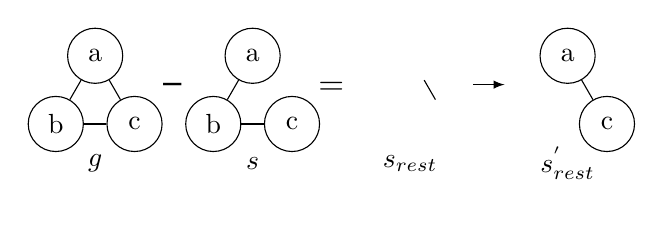
\begin{tikzpicture}[scale=1.0]
%[every node/.style={draw,circle}]
\tikzstyle{line} = [draw,-latex]
\tikzstyle{every node}=[draw,shape=circle,minimum size=0.7cm];
\colorlet{invisible}{white}
\colorlet{visible}{black}
%\tikzstyle{every label}=[text height=10pt];
\begin{scope}[xshift=0cm]
%\draw[help lines] (-1,-6) grid (10,6);
  \node (a) at (60:1cm) {a};
  \node (b) at (0:0cm)  {b};
  \node (c) at (0:1cm)  {c};
  	 \node [draw=none] (minus)  at   (1.5,.5){\scalebox{2.5}[1.5]{-} };
  	 \node [draw=none] (EdgeCutting) at (.5,-.5) {$g$};% edge cutting label

  \foreach \from/\to in {a/b,b/c,c/a}
    \draw (\from) -- (\to);
\end{scope}
\begin{scope}[xshift=2cm]
  \node (a) at (60:1cm) {a};
  \node (b) at (0:0cm)  {b};
   \node (c) at (0:1cm)  {c};
     \node [draw=none] (minus)  at   (1.5,.45){\scalebox{1.2}[1.2]{=} };
 	 \node [draw=none] (EdgeCutting) at (.5,-.5) {$s$};%sharedvertices label
  
  \foreach \from/\to in {a/b,b/c}
    \draw (\from) -- (\to);
\end{scope}
\begin{scope}[xshift=4cm]
  \node[color=invisible] (a) at (60:1cm) {a};
  \node[color=invisible] (c) at (0:1cm)  {c};
    \node [draw=none] (EdgeCutting) at (.5,-.5) {$s_{rest}$};
    \path[line] (1.3,0.5) -- (1.7,0.5);

  \foreach \from/\to in {a/c}
    \draw (\from) -- (\to);
\end{scope}
\begin{scope}[xshift=6cm]
  \node (a) at (60:1cm) {a};
  \node (c) at (0:1cm)  {c};
  \node [draw=none] (EdgeCutting) at (.5,-.5) {$s_{rest}^{'}$};

  \foreach \from/\to in {c/a}
    \draw (\from) -- (\to);
\end{scope}
\end{tikzpicture}

\end{document}

\caption{A case where decomposition of subgraph by partitioning vertices (cutting edges) is not feasible \label{fig:fig7} }
\end{figure}

